\section{Mario Kart 64}

\begin{figure}[htbp]
\begin{center}
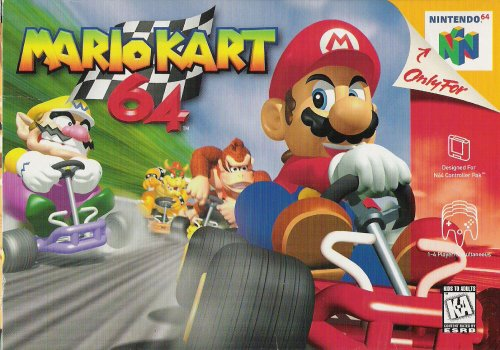
\includegraphics[width=.60\textwidth]{./imagenes/kart1.jpg}
\caption{MarioKart}
\label{Mario Kart}
\end{center}
\end{figure}


\pagecolor{cyan}
\begin{itemize}
\item[Dennise Pintado] \textbf {¿Por qué este juego? \textnormal {Ahora en un mundo donde el poder computacional de las maquinas hacen que todos deseemos  gráficos cada vez más realistas, nos encontramos con gustos algo antiguos u obsoletos pero a mi parecer es como las películas o músicas clásicas, nunca pasaran de moda. Cuando mis padres compraron la consola del  \textcolor{red}{\textsc{Nintendo 64}}} \textnormal {el primer juego a probar fue el MarioKart 64,  con  64 bits de potencia gráfica la inmersión producida en el juego  por estos gráficos 3D llenos de colores, combinado con la iluminación de las carreteras en las que se corría, los efectos de sonido de cada estrella, cascaron, bananas  y el vibrar del control de mando cuando topaba con alguna de estas, me hacían sentir una experiencia de usuario fantástica. Con sus cuatro entradas se podían disfrutar de experiencias multijugador y el  control del juego que se tenía con este  mando era único, ya que su diseño era totalmente adaptable a la mano y daba un control de 360 grados alrededor de la escena que se jugaba.}}

\end{itemize}